%%%%%%%%%%%%%%%%%%%%%%%%%%%%%%%%%%%%%%%%%
% University/School Laboratory Report
% LaTeX Template
% Version 3.0 (4/2/13)
%
% This template has been downloaded from:
% http://www.LaTeXTemplates.com
%
% Original author:
% Linux and Unix Users Group at Virginia Tech Wiki 
% (https://vtluug.org/wiki/Example_LaTeX_chem_lab_report)
%
% License:
% CC BY-NC-SA 3.0 (http://creativecommons.org/licenses/by-nc-sa/3.0/)
%
%%%%%%%%%%%%%%%%%%%%%%%%%%%%%%%%%%%%%%%%%

%----------------------------------------------------------------------------------------
%	PACKAGES AND DOCUMENT CONFIGURATIONS
%----------------------------------------------------------------------------------------

\documentclass{article}
\usepackage[utf8x]{inputenc}
\usepackage[T1]{fontenc}
\usepackage{graphicx}
\usepackage{subfigure}
\usepackage{longtable}
%\usepackage{anysize}
\usepackage{caption}
\usepackage{color}
\usepackage{amssymb}
\usepackage{amsfonts}
\usepackage{amsmath}
\usepackage{bera}% optional: just to have a nice mono-spaced font
\usepackage{listings}
\usepackage{xcolor}

\colorlet{punct}{red!60!black}
\definecolor{background}{HTML}{EEEEEE}
\definecolor{delim}{RGB}{20,105,176}
\colorlet{numb}{magenta!60!black}
\PassOptionsToPackage{hyphens}{url}\usepackage{hyperref}
\hypersetup{
    pdfnewwindow=true,      % links in new window
    colorlinks=true,       % false: boxed links; true: colored links
    %urlcolor=[rgb]{0.45, 0, 0}           % color of external links
}
\definecolor{dkgreen}{rgb}{0,0.6,0}
\definecolor{gray}{rgb}{0.5,0.5,0.5}
\definecolor{mauve}{rgb}{0.58,0,0.82}
\DeclareCaptionFont{white}{\color{white}}
\DeclareCaptionFormat{listing}{\colorbox{gray}{\parbox{\textwidth}{#1#2#3}}}
\captionsetup[lstlisting]{format=listing,labelfont=white,textfont=white}
\usepackage{listings}
\lstset{ %
                basicstyle=\ttfamily,
                keywordstyle=\color{blue}\ttfamily,
                stringstyle=\color{red}\ttfamily,
                commentstyle=\color{green}\ttfamily,
                morecomment=[l][\color{magenta}]{\#}
  basicstyle=\footnotesize,           % the size of the fonts that are used for the code
  numbers=left,                   % where to put the line-numbers
  numberstyle=\tiny\color{gray},  % the style that is used for the line-numbers
  stepnumber=1,                   % the step between two line-numbers. If it's 1, each line 
                                  % will be numbered
  numbersep=5pt,                  % how far the line-numbers are from the code
  backgroundcolor=\color{white},      % choose the background color. You must add \usepackage{color}
  showspaces=false,               % show spaces adding particular underscores
  showstringspaces=false,         % underline spaces within strings
  showtabs=false,                 % show tabs within strings adding particular underscores
  %frame=single,                   % adds a frame around the code
  rulecolor=\color{black},        % if not set, the frame-color may be changed on line-breaks within not-black text (e.g. commens (green here))
  tabsize=2,                      % sets default tabsize to 2 spaces
  captionpos=t,                   % sets the caption-position to bottom
  breaklines=true,                % sets automatic line breaking
  breakatwhitespace=false,        % sets if automatic breaks should only happen at whitespace
  title=\lstname,                   % show the filename of files included with \lstinputlisting;
                                  % also try caption instead of title
  keywordstyle=\color{blue},          % keyword style
  commentstyle=\color{dkgreen},       % comment style
  stringstyle=\color{mauve},         % string literal style
  escapeinside={\%*}{*)},            % if you want to add a comment within your code
  morekeywords={*,...}               % if you want to add more keywords to the set
}
\lstdefinelanguage{json}{
    basicstyle=\normalfont\ttfamily,
    numbers=left,
    numberstyle=\scriptsize,
    stepnumber=1,
    numbersep=8pt,
    showstringspaces=false,
    breaklines=true,
    %frame=lines,
    %backgroundcolor=\color{background},
    literate=
     *{0}{{{\color{numb}0}}}{1}
      {1}{{{\color{numb}1}}}{1}
      {2}{{{\color{numb}2}}}{1}
      {3}{{{\color{numb}3}}}{1}
      {4}{{{\color{numb}4}}}{1}
      {5}{{{\color{numb}5}}}{1}
      {6}{{{\color{numb}6}}}{1}
      {7}{{{\color{numb}7}}}{1}
      {8}{{{\color{numb}8}}}{1}
      {9}{{{\color{numb}9}}}{1}
      {:}{{{\color{punct}{:}}}}{1}
      {,}{{{\color{punct}{,}}}}{1}
      {\{}{{{\color{delim}{\{}}}}{1}
      {\}}{{{\color{delim}{\}}}}}{1}
      {[}{{{\color{delim}{[}}}}{1}
      {]}{{{\color{delim}{]}}}}{1},
}

\setlength\parindent{0pt} % Removes all indentation from paragraphs

\renewcommand{\labelenumi}{\alph{enumi}.} % Make numbering in the enumerate environment by letter rather than number (e.g. section 6)

%\usepackage{times} % Uncomment to use the Times New Roman font

%----------------------------------------------------------------------------------------
%	DOCUMENT INFORMATION
%----------------------------------------------------------------------------------------

\title{
\begin{figure}[ht]
\begin{center}

\includegraphics[scale=0.6]{./common-images/unipd_logo.pdf}
\end{center}
\end{figure}
LiES \\ Linear Equations Solver \\ Sistemi con vincoli \\\vspace{10mm} \textbf{Manuale utente}\\\vspace{0.4cm}
\Large{Anno Accademico 2012/2013}}

\author{Sebastiano \textsc{Gottardo}, Marco \textsc{Ziccardi}\\
Corso di studi in Informatica\\
Dipartimento di Matematica\\
Università degli Studi di Padova\\
Email: dextorer@gmail.com, marco.ziccard@gmail.com }

\date{\today} % Date for the report

\begin{document}

\maketitle % Insert the title, author and date

%\begin{center}
%\begin{tabular}{l r}
%Date Performed: & January 1, 2012 \\ % Date the experiment was performed
%Partners: & Marco Ziccardi \\ % Partner names
%& Sebastiano Gottardo \\
%\end{tabular}
%\end{center}

% If you wish to include an abstract, uncomment the lines below
% \begin{abstract}
% Abstract text
% \end{abstract}

\newpage
\tableofcontents
\newpage

%----------------------------------------------------------------------------------------
%	SECTION 1
%----------------------------------------------------------------------------------------

\section{Introduzione}
\label{sec:introduzione}

Questo documento illustra il funzionamento di LiES (\textit{Linear Equations Solver}) in tutte le sue componenti. La stuttura del documento e' la seguente: Sezione~\ref{sec:requisiti} elenchera' le componenti di sistema necessarie al corretto funzionamento di LiES, mentre in Sezione~\ref{sec:installazione_avvio} verra' spiegato come avviare il software. Dopo aver mostrato la schermata principale in Sezione~\ref{sec:struttura}, le successive sezioni (Sezione~\ref{sec:generazione}, Sezione~\ref{sec:salvataggio}, Sezione~\ref{sec:caricamento}, Sezione~\ref{sec:soluzione}) illustrano rispettivamente le quattro funzioni principali che LiES mette a disposizione: generazione, salvataggio, caricamento e soluzione.

%----------------------------------------------------------------------------------------
%	SECTION 2
%----------------------------------------------------------------------------------------

\section{Requisiti}
\label{sec:requisiti}

Il funzionamento di LiES si basa su due requisiti fondamentali a livello di sistema operativo. Tali requsiti sono elencati di seguito:

\begin{itemize}
	\item JVM/JRE, con versione 6 o superiore - questo requisito e' richiesto in quanto la UI (\textit{User Interface}) e' scritta in linguaggio Java
	\item Compilatore C (e.g., gcc) - richiesto per la compilazione del risolutore
\end{itemize}

Il soddisfacimento dei sopracitati requisiti garantisce il pieno funzionamento di LiES.

%----------------------------------------------------------------------------------------
%	SECTION 3
%----------------------------------------------------------------------------------------

\section{Installazione ed avvio}
\label{sec:installazione_avvio}

LiES viene distribuito attraverso un comodo archivio in formato ZIP, che contiene al suo interno due file:
\begin{itemize}
	\item {\emph{LiES.jar}} - archivio in formato JAR che contiene il software
	\item {\emph{init\_script.sh}} - script di inizializzazione e di avvio
\end{itemize}

Per avviare LiES, e' sufficiente estrarre i contenuti dell'archivio ZIP e lanciare lo script \verb+init_script.sh+, il quale effettuera' automaticamente le seguenti operazioni:
\begin{enumerate}
	\item Estrazione della cartella \textit{csolver} dall'archivio LiES.jar
	\item Compilazione del risolutore, semplificata dalla presenza di un \verb+Makefile+
	\item Copia dell'eseguibile nella cartella principale
	\item Eliminazione della cartella \textit{csolver}
	\item Esecuzione del software tramite avvio dell'archivio JAR LiES.jar
\end{enumerate}

A questo punto LiES sara' avviato e pronto all'uso.

%----------------------------------------------------------------------------------------
%	SECTION 4
%----------------------------------------------------------------------------------------

\section{Struttura}
\label{sec:struttura}

La schermata principale di LiES e' riportata in Figura~\ref{fig:struttura}. I numeri fanno riferimento a diversi settori dell'interfaccia, descritti di seguito. Di nuovo, per semplicita' di esposizione si fara' riferimento ai sistemi di equazioni lineari trattati da LiES con il termine CSP.

\begin{figure}[htp!]
	\centering
	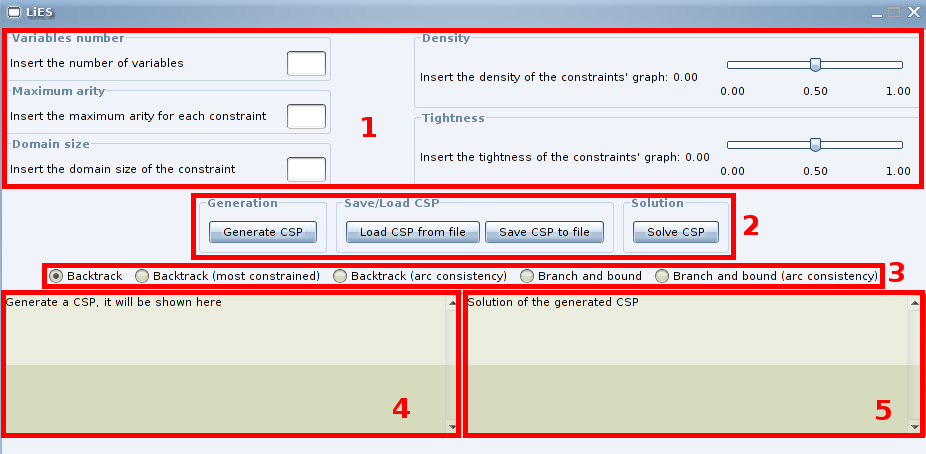
\includegraphics[scale=.4]{ug-images/structure.png}
	\caption{Struttura della schermata principale di LiES.}
	\label{fig:struttura}
\end{figure}

\subsection{1 - Parametri di generazione} 

Questo pannello contiene tutti i parametri che l'utente puo' configurare per generare un sistema di equazioni lineari. Tali parametri fanno riferimento a quelli illustrati nella specifica tecnica: numero di variabili per ciascun vincolo, arieta' (massima) di ciascun vincolo, dimensione del dominio di ciascuna variabile, densita' e strettezza dei vincoli.

\subsection{2 - Pannello dei pulsanti}

Da questo pannello e' possibile operare le varie funzionalita' di LiES. Piu' in dettaglio, e' possibile generare un nuovo sistema di equazioni lineari (se i parametri sono stati opportunamente configurati); e' altresi' possibile salvare un sistema su file e caricarne uno precedentemente salvato. Infine, posto che sia stato generato un problema o sia stato caricato da un file, e' possibile farlo risolvere attraverso l'opportuno pulsante.

\subsection{3 - Metodo di risoluzione}

Questo pannello permette all'utente di scegliere la tecnica di risoluzione che LiES utilizzera' con il sistema di equazioni lineari attuale.

\subsection{4 - Pannello di visualizzazione del sistema}

Una volta generato un sistema di equazioni, oppure una volta che questo e' stato caricato da un file, viene visualizzato in questo pannello.

\subsection{5 - Pannello di visualizzazione della soluzione}

Ogni volta che il risolutore viene invocato, il risultato della sua computazione viene riportato in questo pannello. Sara' quindi possibile scorrere tutte le operazioni fatte dal risolutore, visualizzare la soluzione (se esistente) e alcune altre statistiche (e.g., tempo impiegato).

%----------------------------------------------------------------------------------------
%	SECTION 5
%----------------------------------------------------------------------------------------

\section{Generazione}
\label{sec:generazione}

La generazione di un nuovo sistema di equazioni lineari prevede che l'utente inserisca dei parametri di configurazione nell'apposito pannello, riportato in Figura~\ref{fig:parametri}.

\begin{figure}[htp!]
	\centering
	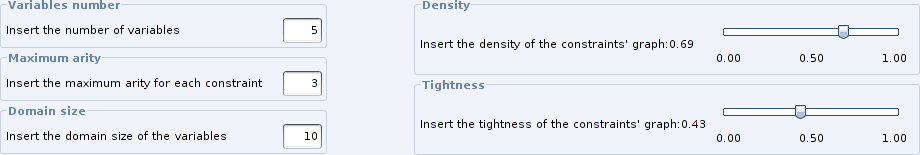
\includegraphics[scale=.4]{ug-images/parameters.png}
	\caption{Pannello di configurazione dei parametri di generazione.}
	\label{fig:parametri}
\end{figure}

Una volta che il pulsante ``Generate CSP'' e' stato premuto, il generatore random di LiES controlla che tutti i parametri abbiano un valore, li raccoglie e li utilizza per creare un nuovo sistema di equazioni lineari. Il risultato e' visualizzabile sull'apposito pannello, come mostrato in Figura~\ref{fig:visualizzazione}.

\begin{figure}[htp!]
	\centering
	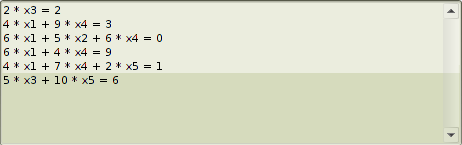
\includegraphics[scale=.5]{ug-images/system.png}
	\caption{Visualizzazione di un sistema di equazioni lineari generato casualmente.}
	\label{fig:visualizzazione}
\end{figure}

Sebbene il problema venga generato, salvato e caricato utilizzando una struttura in formato JSON, la sua visualizzazione viene preceduta da una fase di elaborazione al fine di offrire una rappresentazione piu' comprensibile del problema in questione. Le equazioni saranno infatti perfettamente leggibili e in un formato consono all'utente.

%----------------------------------------------------------------------------------------
%	SECTION 6
%----------------------------------------------------------------------------------------

\section{Salvataggio}
\label{sec:salvataggio}

Il salvataggio su file di un sistema di equazioni lineari e' reso possibile dall'apposito pulsante. Una volta premuto, l'utente disporra' di una finestra come quella mostrata in Figura~\ref{fig:finestra_salvataggio}: una volta scelto il percorso e assegnato un nome al file, la conferma dell'utente mostrera il messaggio di Figura~\ref{fig:conferma_salvataggio}, che informa l'utente dell'avvenuto salvataggio.

\begin{figure}[htp!]
\centering
	\subfigure[SaveDialog]
	{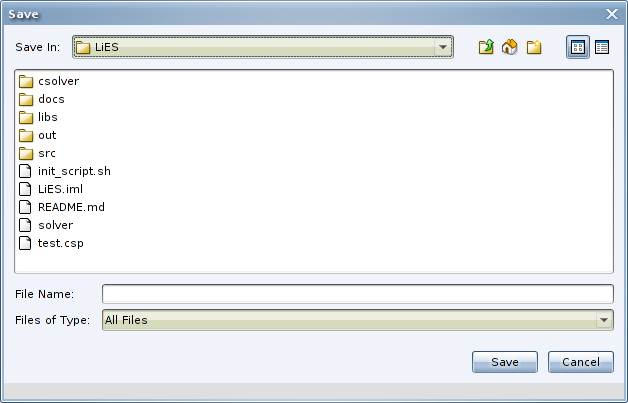
\includegraphics[width=8cm]{ug-images/save-dialog.png}\label{fig:finestra_salvataggio}}
	\subfigure[ConfirmDialog]
	{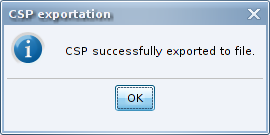
\includegraphics[width=4cm]{ug-images/save-confirm.png}\label{fig:conferma_salvataggio}}
	\caption{Finestre di salvataggio di un CSP su file.}
	\label{fig:salvataggio}
\end{figure}

%----------------------------------------------------------------------------------------
%	SECTION 7
%----------------------------------------------------------------------------------------

\section{Caricamento}
\label{sec:caricamento}

L'operazione di caricamento, similmente all'operazione di salvataggio, mostra all'utente la finestra di scelta di un file riportata in Figura~\ref{fig:caricamento}: attraverso questa, l'utente puo' selezionare un sistema di equazioni lineari precedentemente salvato e caricarlo su LiES. 

\begin{figure}[htp!]
	\centering
	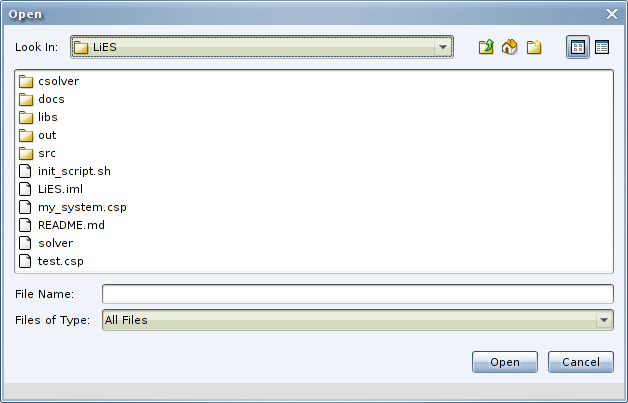
\includegraphics[scale=.5]{ug-images/load-dialog.png}
	\caption{Finestra di caricamento da file di un CSP precedentemente salvato.}
	\label{fig:caricamento}
\end{figure}

Tuttavia, a differenza dell'operazione di salvataggio, non viene mostrato nessun messaggio di conferma. L'utente e' in grado di stabilire se il sistema di equazioni e' stato caricato con successo se questo compare nell'apposito pannello di visualizzazione (in basso a sinistra). Inoltre, si fa presente che poiche' esso e' stato generato casualmente, i parametri originali che ne hanno portato alla creazione non sono riportati nel pannello di configurazione, che viene quindi resettato.

\section{Soluzione}
\label{sec:soluzione}

\begin{figure}[htp!]
	\centering
	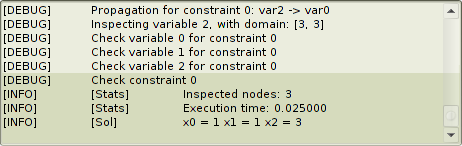
\includegraphics[scale=.5]{ug-images/solution.png}
	\caption{Pannello che mostra la soluzione di un sistema di equazioni lineari generato casualmente.}
	\label{fig:soluzione}
\end{figure}

L'operazione di risoluzione permette all'utente di visualizzare una soluzione, se esiste, di un sistema di equazioni lineari generato casualmente al momento o caricato da un file precedentemente salvato. La scelta della tecnica che il risolutore utilizzera' per calcolare la soluzione e' lasciata all'utente, che potra' scegliere tra cinque opzioni. Una premuto il pulsante che avvia la risoluzione, nell'apposito pannello compariranno i messaggi del risolutore, che terminera' o con la soluzione oppure con un fallimento. In entrambi i casi, sara' possibile visualizzare alcune statistiche sul calcolo (e.g., tempo impiegato) e sara' possibile ripercorrere tutti i passi effettuati nel calcolo della soluzione. Un esempio di soluzione e' visibile in Figura~\ref{fig:soluzione}.

%----------------------------------------------------------------------------------------


\end{document}
